%\subsection{Durchführung}
%\label{sec:Durchführung}
\section{Wheatstonebrücke}
\subsection{Durchführung}
Abbildung \ref{fig:1} zeigt den systematischen Aufbau einer Wheatstonebrücke.
\begin{figure}[H]
  \centering
  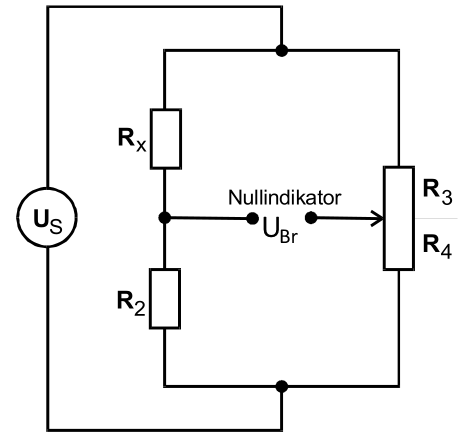
\includegraphics[height=6cm]{wheat.png}
  \caption{Wheatstonebrücke \cite{sample}}
  \label{fig:1}
\end{figure}
Sie besteht aus jeweils zwei parallel zueinander geschalteten Widerständen $R_x$ und $R_3$, und $R_2$ und $R_4$.
Es wird die Potentialdifferenz $U_{\text{br}}$ zwischen den beiden Punkten nach jeweils dem ersten Widerstand abgegriffen.
Bei dieser mit Wechselstrom betriebenen Schaltung wird das Verhältnis von $R_3$ zu $R_4$ nun solange variiert bis die Brückenspannunng $U_{\text{Br}}$ ihr Minimum erreicht hat.
Somit kann $R_x$ bestimmt werden.
Es werden zwei unbekannte Widerstände $R_x$ mit jeweils drei verschiedenen $R_2$ ermittelt.
\subsection{Auswertung}
\begin{table}
  \centering
  \caption{Messdaten R = Wert14}
  \label{tab:1}
  \sisetup{table-format=3.4}
  \begin{tabular}{c c c c}
    \toprule
    {$R_2 [\si{\ohm}]$} & {$\increment R_2 [\si{\ohm}]$} & {$\frac{R_3}{R_4}$} & {$\increment \frac{R_3}{R_4}$} \\
    \midrule
    \input{build/wheat1tabelle.tex}
    \bottomrule
  \end{tabular}
\end{table}


\begin{table}
  \centering
  \caption{Messdaten R = Wert11}
  \label{tab:2}
  \sisetup{table-format=3.4}
  \begin{tabular}{c c c c}
    \toprule
    {$R_2 [\si{\ohm}]$} & {$\increment R_2 [\si{\ohm}]$} & {$\frac{R_3}{R_4}$} & {$\increment \frac{R_3}{R_4}$} \\
    \midrule
    \input{build/wheat2tabelle.tex}
    \bottomrule
  \end{tabular}
\end{table}


\begin{align}
  R_{14}   &= \input{build/wheat/wheat.R14m.tex}\\
  R_{11}   &= \input{build/wheat/wheat.R11m.tex}
\end{align}

\section{Kapazitätsmessbrücke}
\subsection{Durchführung}
Mit der Kapazitätsmessbrücke kann die Kapazität und der Widerstand eines unbekannten Kondensatorelements berechnet werden.
Die Abbildung \ref{fig:2} zeigt eine solche Schaltung.
\begin{figure}[H]
  \centering
  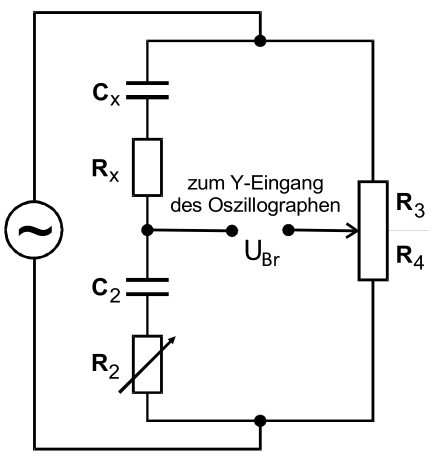
\includegraphics[height=6cm]{kapa.png}
  \caption{Kapazitätsmessbrücke \cite{sample}}
  \label{fig:2}
\end{figure}
Sie unterscheidet sich von der Wheatstonebrücke nur darin, dass hier anstelle von $R_x$ eine unbekannte R/C-Kombination oder eben nur ein unbekannter Kondensator eingebaut und ermittelt wird.
Zusätzlich wird mit einem festen Kondensator $C_2$ und einem variablen Widerstand $R_2$ abgegelichen.
Es werden nun $R_2$ und das Verhältnis von $R_3$ und $R_4$ solange nacheinander variiert bis das Minimum der Brückenspannung $U_{\text{Br}}$ auf dem Oszilloskop beobachtet wird.
Auf diese Weise werden die Kapazitäten und Widerstände einer R/C-Kombination, sowie von zwei unbekannten Kondensatoren bestimmt.
Es wird jeweils dreimal mit verschiedenen Kondensatoren $C_2$ gemessen.
\subsection{Auswertung}
\begin{table}
  \centering
  \caption{Messdaten R/C = Wert8}
  \label{tab:3}
  \sisetup{table-format=3.4}
  \begin{tabular}{c c c c c c}
    \toprule
    {$C_2 [\si{\nano\farad}]$} & {$\increment C_2 [\si{\nano\farad}]$} & {$R_2 [\si{\ohm}]$} & {$\increment R_2 [\si{\ohm}]$} & {$\frac{R_4}{R_3}$} & {$\increment \frac{R_4}{R_3}$} \\
    \midrule
    \input{build/kapa1tabelle.tex}
    \bottomrule
  \end{tabular}
\end{table}
\begin{table}
  \centering
  \caption{Messdaten C = Wert3}
  \label{tab:4}
  \sisetup{table-format=3.4}
  \begin{tabular}{c c c c c c}
    \toprule
    {$C_2 [\si{\nano\farad}]$} & {$\increment C_2 [\si{\nano\farad}]$} & {$R_2 [\si{\ohm}]$} & {$\increment R_2 [\si{\ohm}]$} & {$\frac{R_4}{R_3}$} & {$\increment \frac{R_4}{R_3}$} \\
    \midrule
    \input{build/kapa2tabelle.tex}
    \bottomrule
  \end{tabular}
\end{table}
\begin{table}
  \centering
  \caption{Messdaten C = Wert1}
  \label{tab:5}
  \sisetup{table-format=3.4}
  \begin{tabular}{c c c c c c}
    \toprule
    {$C_2 [\si{\nano\farad}]$} & {$\increment C_2 [\si{\nano\farad}]$} & {$R_2 [\si{\ohm}]$} & {$\increment R_2 [\si{\ohm}]$} & {$\frac{R_4}{R_3}$} & {$\increment \frac{R_4}{R_3}$} \\
    \midrule
    \input{build/kapa3tabelle.tex}
    \bottomrule
  \end{tabular}
\end{table}

\section{Induktivitätsmessbrücke}
\subsection{Durchführung}
Die Induktivitätsmessbrücke, dargestellt in Abbildung \ref{fig:3}, funktioniert im Prinzip genauso wie die Kapazitätsmessbrücke \ref{fig:2}.
\begin{figure}[H]
  \centering
  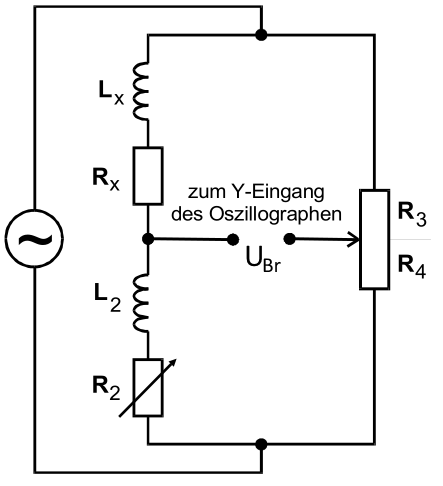
\includegraphics[height=6cm]{indu.png}
  \caption{Induktivitätsmessbrücke \cite{sample}}
  \label{fig:3}
\end{figure}
Anstelle der Kondensatoren werden hier jedoch die Spule $L_2$ und eine L/R-Kombination eingebaut.
Es gilt das selbe Messverfahren wie bei der Kapazitätsmessbrücke, um diesmal die Werte von nur einer unbekannten L/R-Kombination zu ermitteln.
$L_2$ wird dabei zweimal variiert.
\subsection{Auswertung}
\begin{table}
  \centering
  \caption{Messdaten L/R = Wert19}
  \label{tab:6}
  \sisetup{table-format=3.4}
  \begin{tabular}{c c c c c c}
    \toprule
    {$L_2 [\si{\milli\henry}]$} & {$\increment L_2 [\si{\milli\henry}]$} & {$R_2 [\si{\ohm}]$} & {$\increment R_2 [\si{\ohm}]$} & {$\frac{R_3}{R_4}$} & {$\increment \frac{R_3}{R_4}$} \\
    \midrule
    \input{build/indu1tabelle.tex}
    \bottomrule
  \end{tabular}
\end{table}



\section{Maxwell-Brücke}
\subsection{Durchführung}
Da bei der Induktivitätsmessbrücke auf eine Spule zur Berechnung der unbekannten Induktivität zurückgegriffen wird, diese aber zumeist bei niedrigen Frequenzen hohe Verluste besitzt, ist es besser anstelle einer Spule einen möglichst verlustarmen Kondensator zu verwenden.
Dies wird bei der Maxwell-Brücke, Abbildung \ref{fig:4}, realisiert.
\begin{figure}[H]
  \centering
  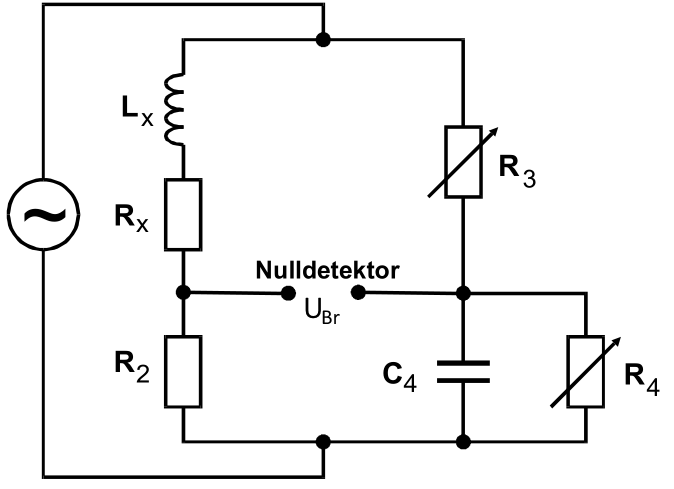
\includegraphics[height=6cm]{max.png}
  \caption{Maxwell-Brücke \cite{sample}}
  \label{fig:4}
\end{figure}
Die Abgleichelemente sind hier die variablen Widerstände $R_3$ und $R_4$, wobei der Kondensator $C_4$ parallel zu $R_3$ geschaltet wird.
Dabei soll die selbe L/R-Kombination untersucht werden, indem $R_3$ und $R_4$ nacheinander variiert werden, sodass die Brückenspannung $U_{\text{Br}}$ minimal wird.
Es wird dreimal mit verschiedenen Widerständen $R_2$ gemessen.
\subsection{Auswertung}
\begin{table}
  \centering
  \caption{Messdaten C = Wert1}
  \label{tab:7}
  \sisetup{table-format=3.4}
  \begin{tabular}{c c c c c c c c}
    \toprule
    {$C_4 [\si{\nano\farad}]$} & {$\increment C_4 [\si{\nano\farad}]$} & {$R_3 [\si{\ohm}]$} & {$\increment R_3 [\si{\ohm}]$} & {$R_2 [\si{\ohm}]$} & {$\increment R_2 [\si{\ohm}]$} & {$\frac{R_4}{R_3}$} & {$\increment \frac{R_4}{R_3}$} \\
    \midrule
    \input{build/max1tabelle.tex}
    \bottomrule
  \end{tabular}
\end{table}




\section{Wien-Robinson-Brücke}
\subsection{Durchführung}
Bei den obigen Schaltungen ist ein Abgleich bei beliebigen Frequenzen möglich.
Bei der Wien-Robinson-Brücke \ref{fig:5} hingegen ist ein Abgleich nur bei einer bestimmten Frequenz möglich, die untersucht werden soll.
\begin{figure}[H]
  \centering
  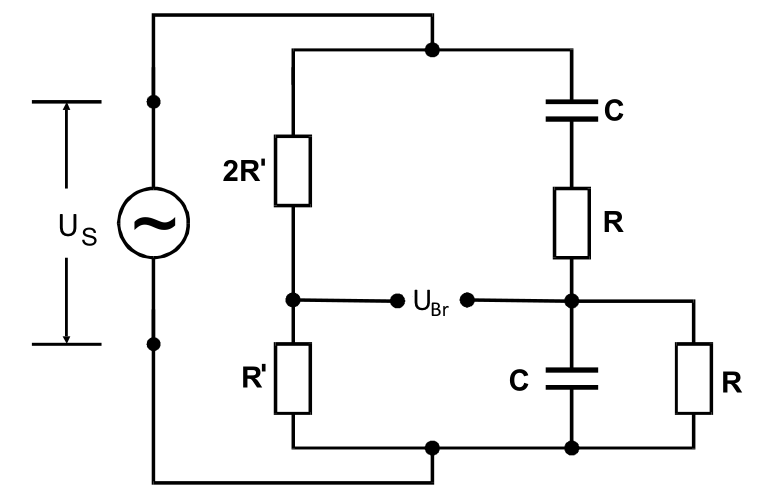
\includegraphics[height=6cm]{wien.png}
  \caption{Wien-Robinson-Brücke \cite{sample}}
  \label{fig:5}
\end{figure}
Dabei wird die Frequenz $v$ der Speisespannung $U_{\text{S}}$ in um die Minimalbrückenspannung kleiner werdenden Abständen variiert und die jeweilige entstehende Brückenspannung $U_{\text{Br}}$ notiert.
Die Frequenz befindet sich in einem Bereich von $\SI{20}{\hertz}$ bis $\SI{30}{\kilo\hertz}$.
\subsection{Auswertung}
\begin{table}
  \centering
  \caption{Messdaten Frequenzmessung}
  \label{tab:8}
  \sisetup{table-format=5.4}
  \begin{tabular}{c c}
    \toprule
    {$v [\si{\hertz}]$} & {$U_{\text{Br}} [\si{\volt}]$} \\
    \midrule
    \input{build/frequenztabelle.tex}
    \bottomrule
  \end{tabular}
\end{table}
